\begin{center}
    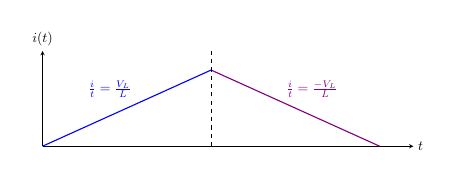
\begin{tikzpicture}
        [
            scale = 0.5,
            >=latex
        ]
        \begin{axis}
            [
                width=11cm,
                height=4cm,
                xmin=0, xmax=11, ymin=0, ymax=5, axis lines=middle,
                x label style={anchor=west},
                xlabel=$t$,
                y label style={anchor=south},
                ylabel=$i(t)$,
                ticks=none
                %grid
            ]
            
            %nodes
            \node                       (m)     at (5,4)        {};
            \node                       (e)     at (10, 0)      {};
            \node[color=blue]           (s1)    at (2, 3)       {$\frac{\diff i}{\diff t} = \frac{V_L}{L}$};
            \node[color=violet]         (s2)    at (8, 3)       {$\frac{\diff i}{\diff t} = \frac{-V_L}{L}$};

            plots
            \addplot[color=blue, thick, domain=0:5]{0.8*x};
            \addplot[color=violet, thick, domain=5:10]{-0.8*x+8};
            \addplot[dashed]coordinates {(5, 0) (5, 5)};
        \end{axis}
        % \node[label={below:\tiny $t = 0$}](t0)    at (0, 0)       {};
    \end{tikzpicture}
\end{center}
